
\chapter{Background}

\section{Processor - Process - Thread}

\myparagraph{Processor}
The processor is the central processing unit of a computer. The processor is also called CPU for short. Each processor can execute exactly one specific instruction set. Examples for known instruction sets are the x86 architecture and the ARM architecture. A processor usually consists of several components. Among others, a processor contains the ALU (arithmetic-logical unit), the MMU (memory management unit), and several other registers. \cite{Tannenbaum:21}
\\
Nowadays processors usually have several cores. \cite{Tannenbaum:87} This means that there are several mini chips on these processors, which can execute instructions independently of each other. Furthermore, many CPUs are capable of multithreading. Multithreading allows a core to remember the state of two threads. This allows the core to switch quickly between them. This is also called pseudo-parallelism.\cite{Tannenbaum:23}
\\
If one wants to increase the performance of a processor, there are two options. Either one increases the individual performance of the cores or one increases the number of cores. Today, the performance of an individual core is close to the limit of what is physically possible. Due to limitations in heat generation, only small increases in performance are possible today. On the other hand, increasing the number of cores is far from the limit. Multi-core systems are not only in demand in the industry but are also available to private individuals. [Citation needed]
If you look at the sales figures of the german computer parts reseller Mindfactory, you can see that most of the sold processors have 4, 6, 8 and even 16 cores. 

\begin{figure}[H]
  \centering
  \begin{subfigure}[b]{1.0\textwidth}
    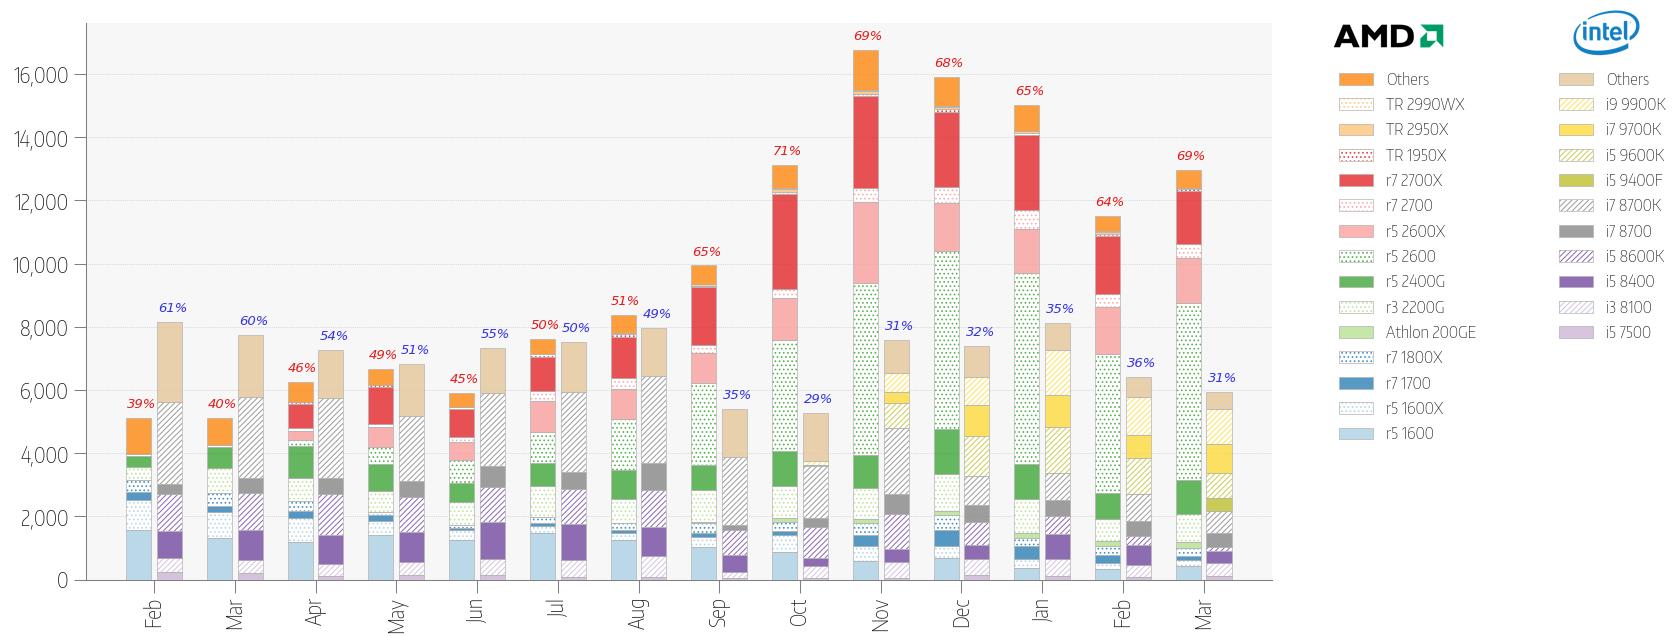
\includegraphics[width=1.0\linewidth]{img/mindfactory-sales2.png}
  \end{subfigure}
  \caption{Mindfactory CPU Sales \cite{forbes:mindfactory:sales}}
  \label{Mindfactory CPU Sales}
\end{figure}

\myparagraph{Process}
A process is a program that is being executed. In the following figure, the relation between a process and a program is presented.

\begin{figure}[H]
  \centering
  \begin{subfigure}[b]{1.0\textwidth}
    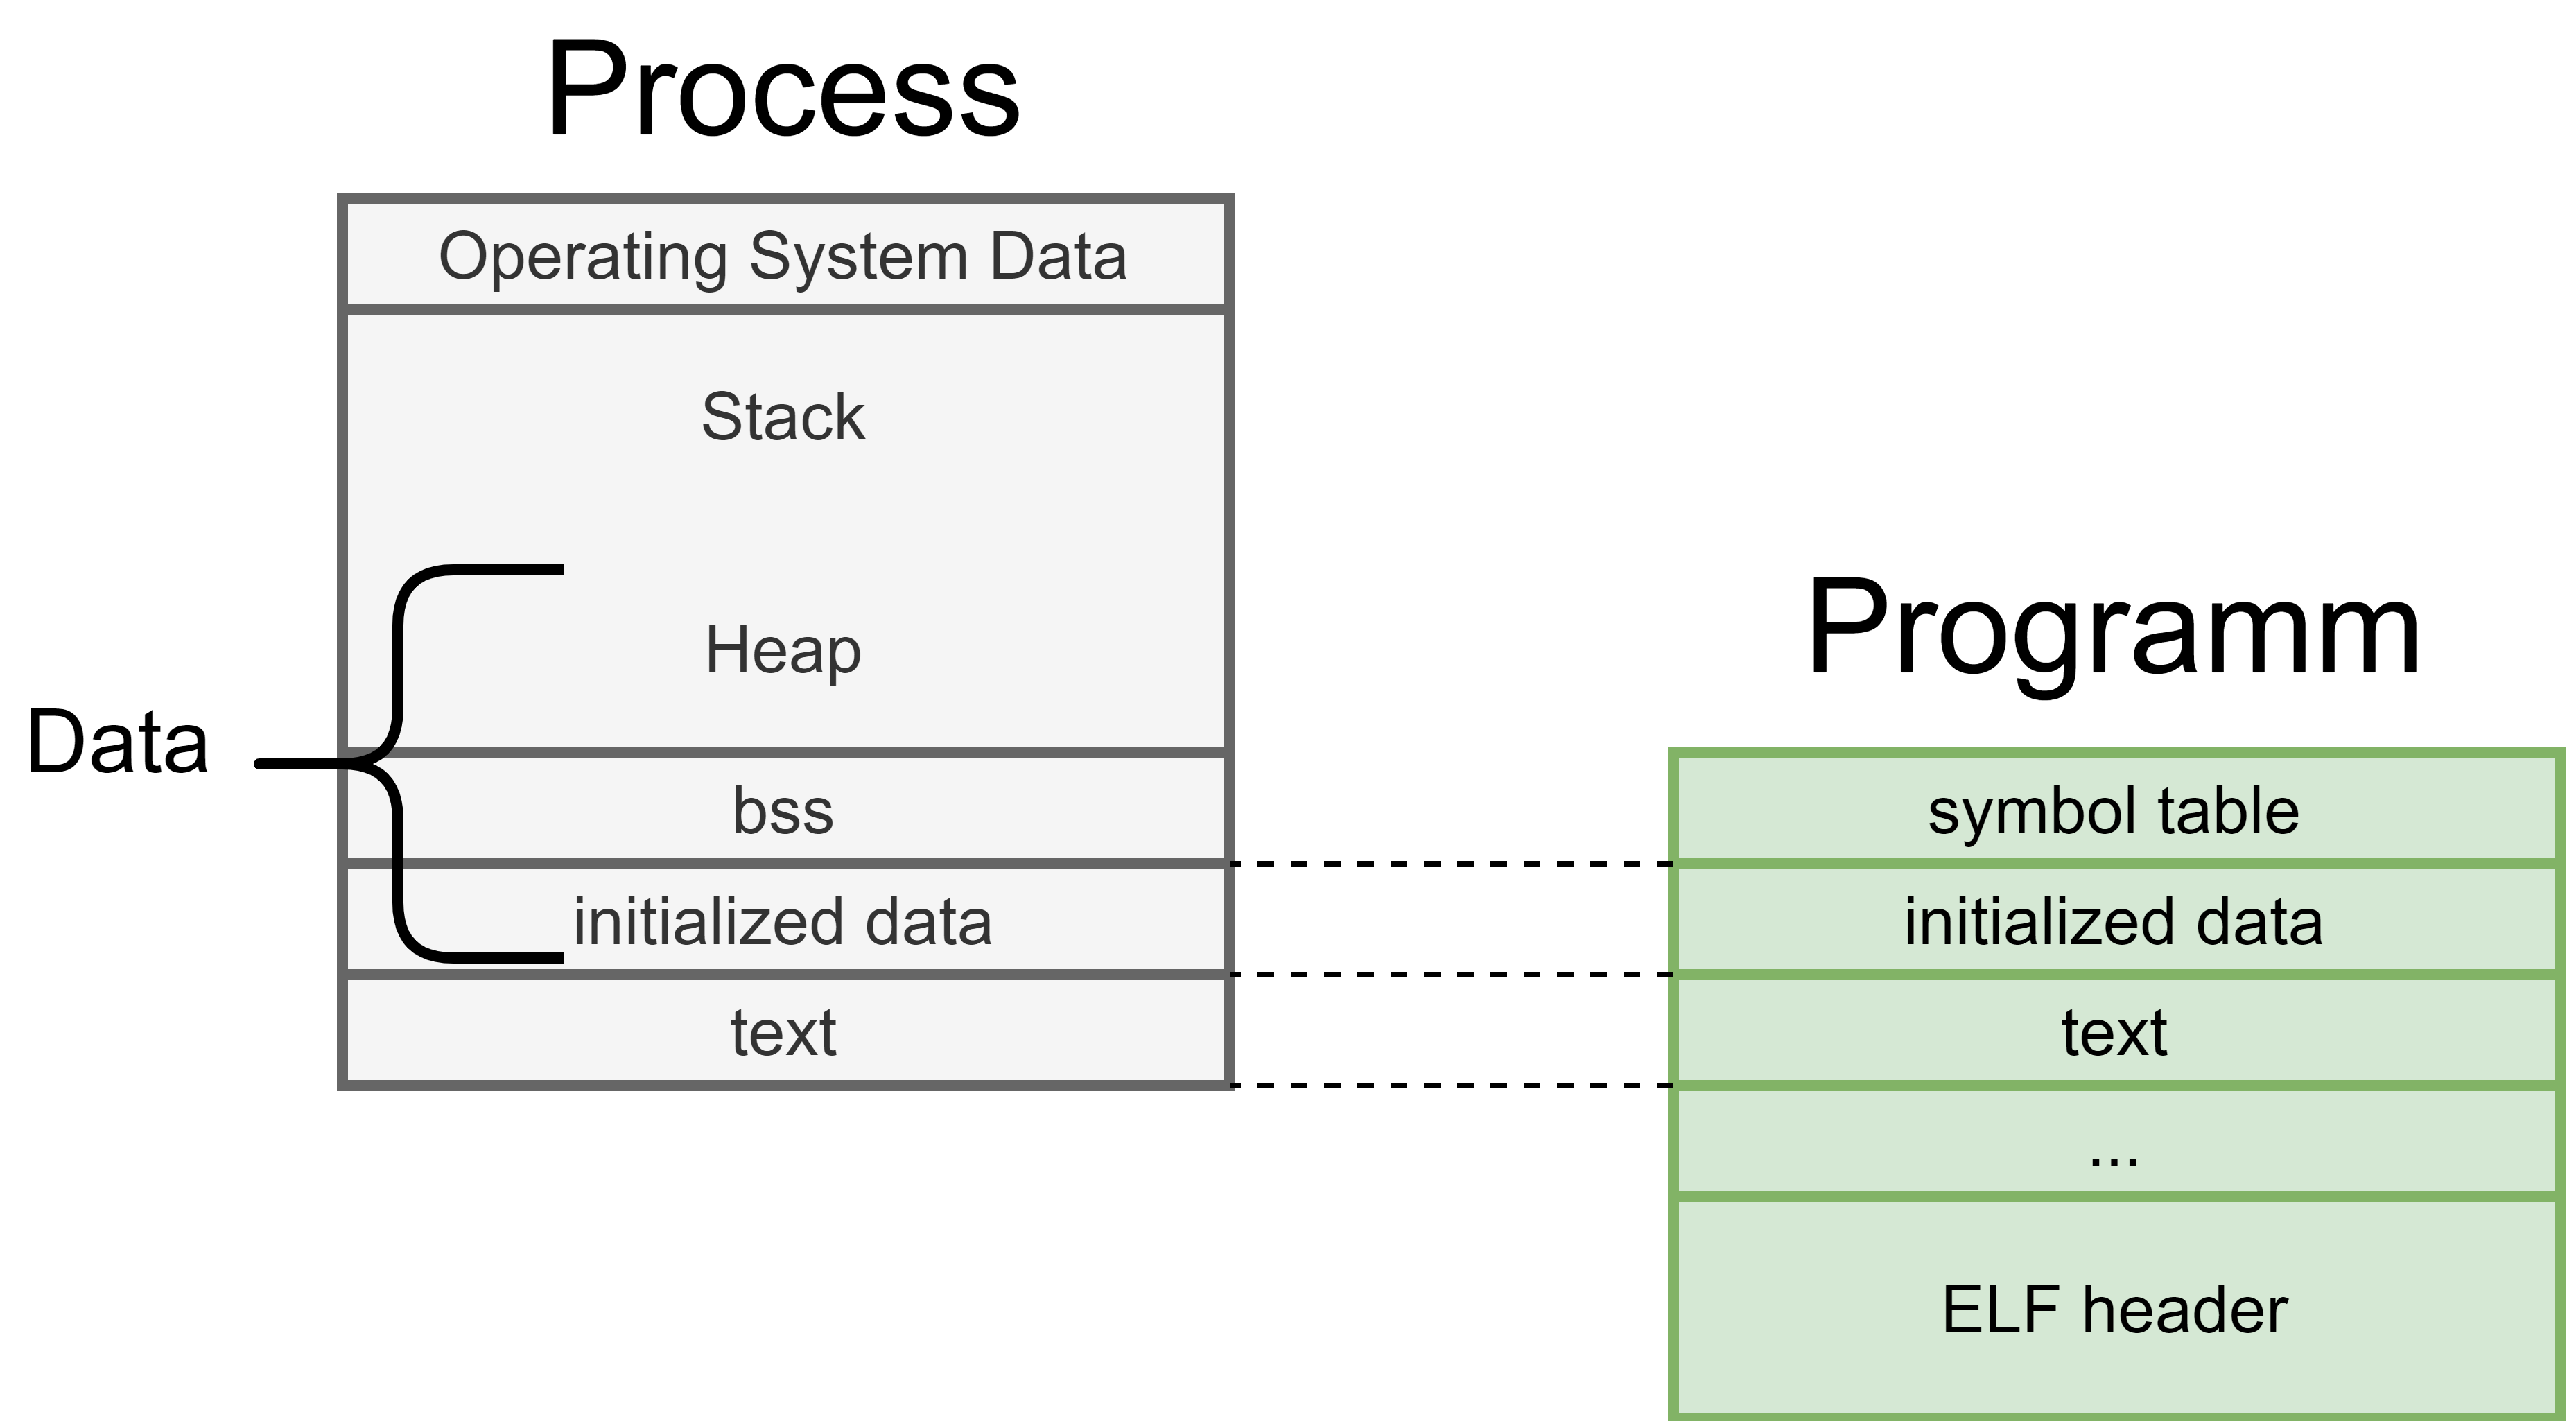
\includegraphics[width=1.0\linewidth]{img/process-program.png}
  \end{subfigure}
  \caption{Process vs Program \cite{Schoettner:bs18:4.5}}
  \label{process-program}
\end{figure}

The segment \textit{text} contains the programcode.
The segment \textit{initialized data} contains initialized global and static variables.
The segment \textit{bss} contains not yet initialized global variables and static variables.
The \textit{heap} is the extension of the \textit{bss}.
The \textit{stack} is used for saving local variables, function parameters and memory areas of register contents.
Both the \textit{stack} and the \textit{heap} will be dynamically extended if needed.\cite{Schoettner:bs18:4.5}
\\
Processes allow a system to process several programs simultaneously. An active process can have three different statuses.
\\
\begin{figure}[H]
  \centering
  \begin{subfigure}[b]{1.0\textwidth}
    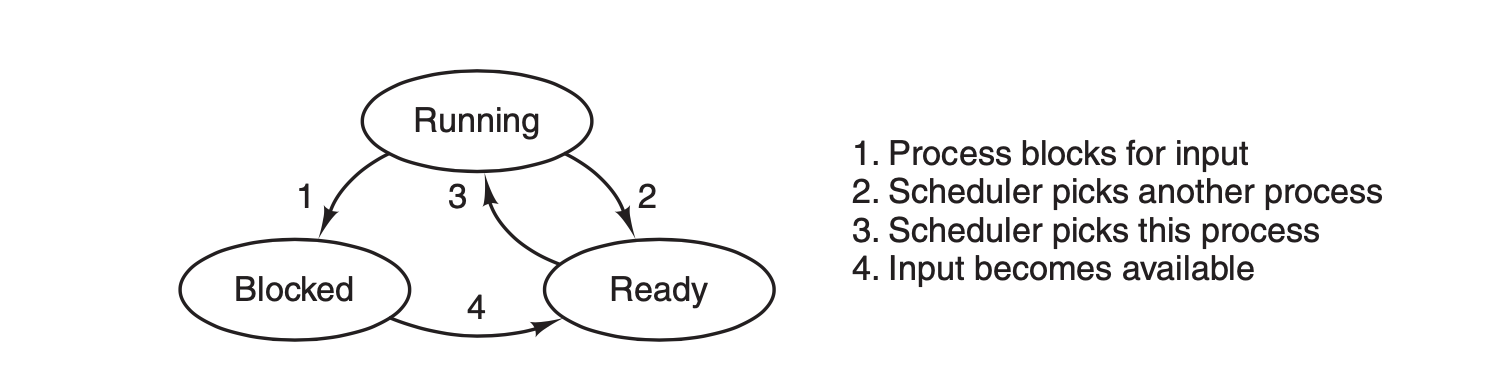
\includegraphics[width=1.0\linewidth]{img/prozess-status.png}
  \end{subfigure}
  \caption{Process Status \cite{Tannenbaum:93}}
  \label{process-status}
\end{figure}

The scheduler plays an important role here. A scheduler is responsible for when a process is processed by the CPU. In UNIX systems, for example, a round-robin scheduler is used. This changes the active process in a predetermined cycle, such as 10-100ms. \cite{Schoettner:bs18:6.6.4}
An active process is a process with the status \textit{Running}. The CPU is then assigned to the process and executes the program of the process. If the CPU is removed from the process by the scheduler, the process is in \textit{Ready} status. The process is then ready to be reassigned to the CPU and is waiting for it. A process can also block. This happens if the process has to wait for a certain input. The process is then in \textit{Blocked} status and will not change to \textit{Ready} status until the input becomes available. \cite{Tannenbaum:93}

\myparagraph{Thread}
A process is heavy. Each process has its own address space and switching between processes takes a lot of time. Therefore threads were created as lightweight processes. Threads are part of a process and therefore they share the same address space. Switching between threads is a lot faster. The following diagram lists the unique items for threads and processes.
\\
\begin{figure}[H]
  \centering
  \begin{subfigure}[b]{0.6\textwidth}
    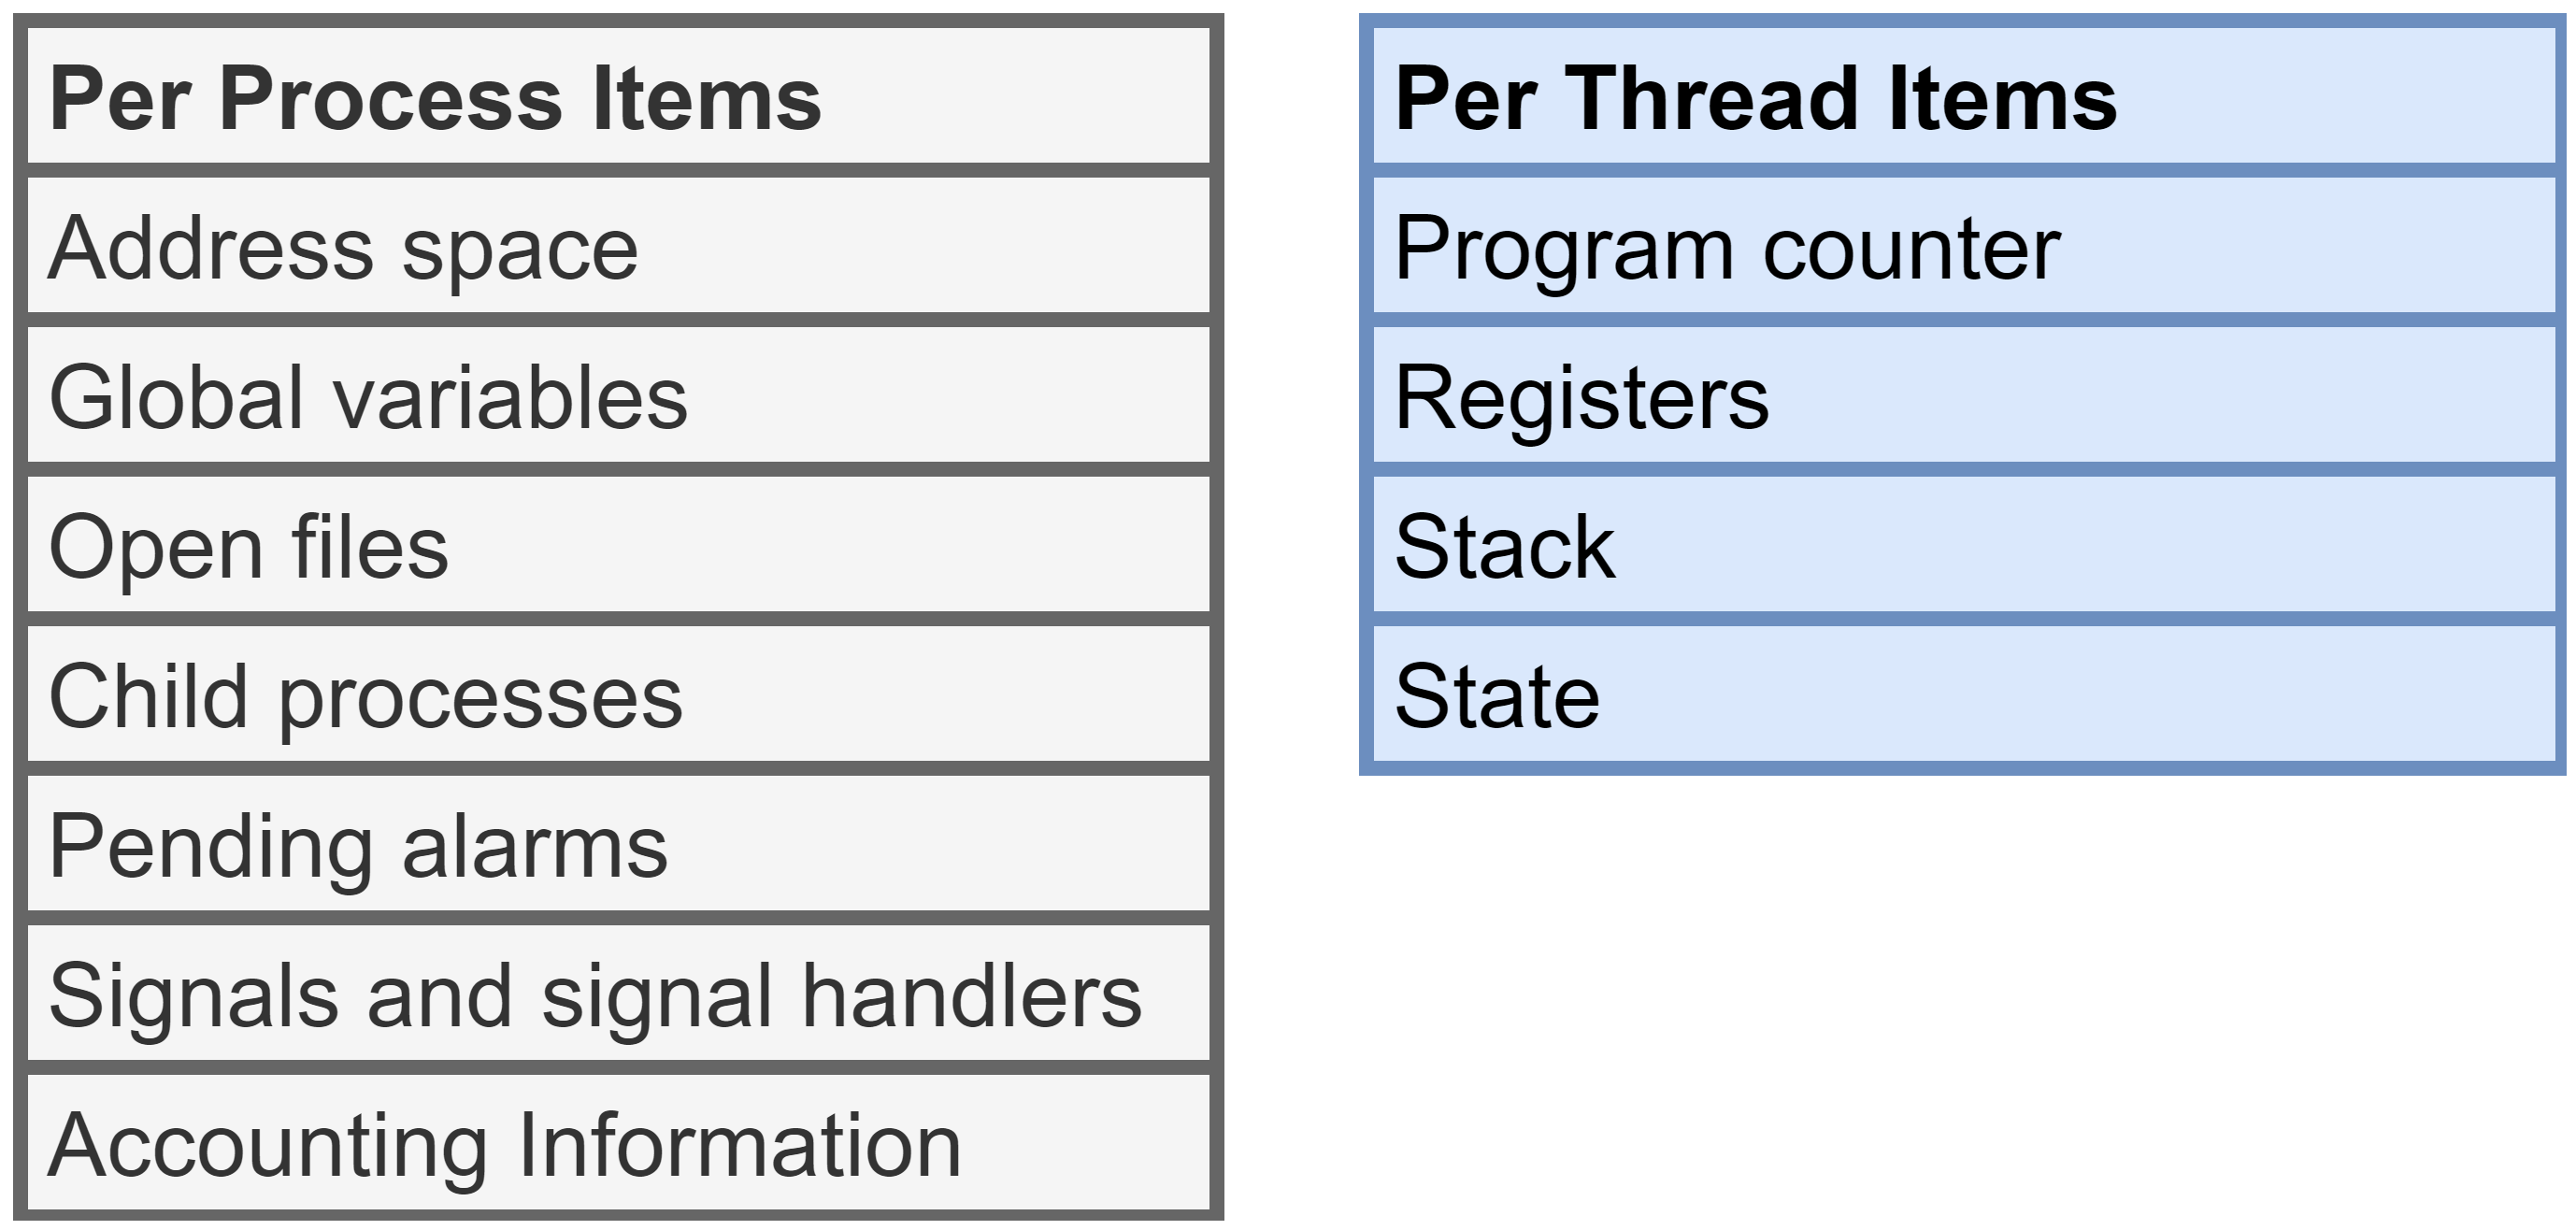
\includegraphics[width=1.0\linewidth]{img/process-thread-items.png}
  \end{subfigure}
  \caption{Process vs Thread \cite{Tannenbaum:104}}
  \label{Process vs Thread}
\end{figure}

Each process can have many threads. The following figure shows the hierarchy of processes and threads.

\begin{figure}[H]
  \centering
  \begin{subfigure}[b]{1.0\textwidth}
    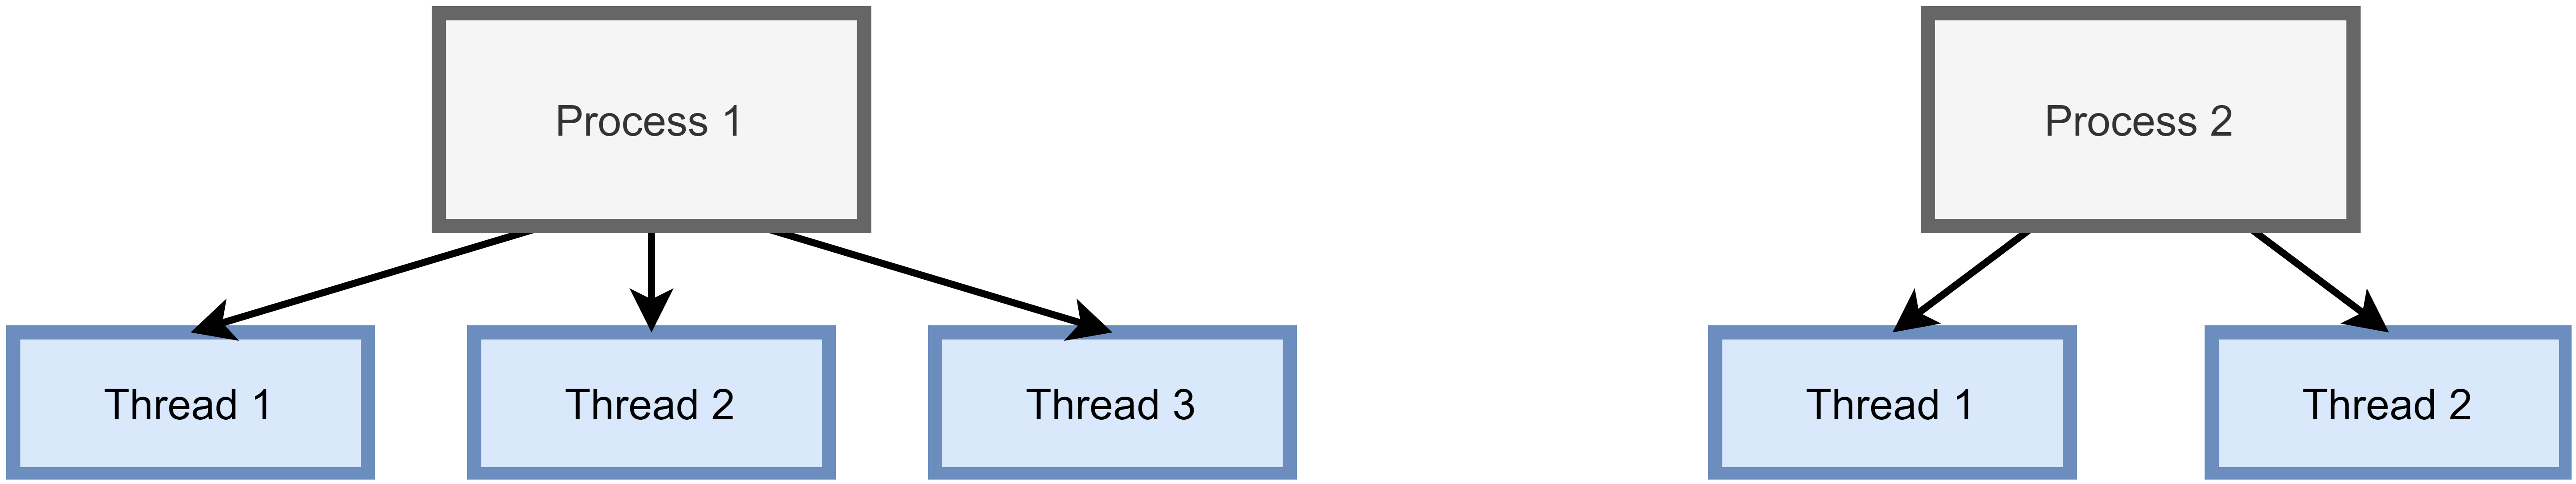
\includegraphics[width=1.0\linewidth]{img/process-thread.png}
  \end{subfigure}
  \caption{Process - Thread - Hierarchy}
  \label{Process - Thread - hierarchy}
\end{figure}
In modern programming, the line between processes and threads gets somewhat blurred, because processes often start with a single thread. Standalone processes without any threads are a thing of the past.
\\
\\
Threads increase CPU efficiency. Whenever a thread has to block, for example, because it has to wait for I/O input, another thread of the same process can quickly continue and make use of the CPU. Constantly switching between processes would be very inefficient.
\\
\\
A distinction is made between two types of threads. Kernel-level threads, which are managed directly by the operating system's scheduler and User-level threads, where the programmer has to do the scheduling himself.\cite{Schoettner:bs18:6.4}

\section{Atomic Functions}
In the context of multithreading a race condition occurs, when multiple threads utilize the same variables. Per default, the result of such a race condition is not deterministic. This is unwanted behavior. The solution is to only allow one thread to access that variable at a time. This can be realized by using a lock variable, which gets set to True whenever one thread tries to access the variable. Once the thread is done, the lock gets released by setting it to False. The immediate problem is, that another race condition occurs. Instead of having a race condition for the old variables, now one has a race condition for the lock. \cite{Schoettner:bs18:7.4}
To fix this, the lock variable has to be set atomically. "An operation acting on shared memory is atomic if it completes in a single step relative to other threads." \cite{Preshing}
\\
\\
In Java, there are multiple implementations of atomic functions. One of them is the VarHandle class. A VarHandle is a reference to a variable. VarHandles support multiple access modes with different functions. In this context, the most important functions are part of the atomic update access modes. An example of such a function would be:
\begin{lstlisting}[language=custom-java]
  public final boolean compareAndSet(Object... args)
\end{lstlisting}
compareAndSet receives two parameters: expectedValue and newValue. It will check whether the current value equals the expectedValue. If that is the case it will set the value to newValue and return True. If not, the value remains unchanged and False is returned.

\section{Intrinsic Functions}
"In compiler theory, an intrinsic function is a function available for use in a given programming language whose implementation is handled specially by the compiler. Typically, it substitutes a sequence of automatically generated instructions for the original function call." \cite{wiki:intrinsics}
\\
\\
OpenJDK provides a descriptive example, using the String::format function. Consider the following code:
\begin{lstlisting}[language=custom-java]
  String name = ...
  int age = ...
  String s = String.format("%s: %d", name, age);
\end{lstlisting}
Without intrinsification this piece of code would be translated to inefficient bytecode.
Using the knowledge that the format specifier is constant, a more efficient translation to bytecode is possible. According to OpenJDK, the more efficient bytecode runs 30-50 times faster than the first one. \cite{OpenJDK:intrinsics}
\\
\\
Intrinsic functions are often abbreviated as intrinsics.


\subsection{C/C++}
There are many different C and C++ compilers. As an example Microsoft's compiler supports intrinsics. In Microsoft's implementation, "if a function is an intrinsic, the code for that function is usually inserted inline, avoiding the overhead of a function call and allowing highly efficient machine instructions to be emitted for that function. An intrinsic is often faster than the equivalent inline assembly, because the optimizer has a built-in knowledge of how many intrinsics behave, so some optimizations can be available that are not available when inline assembly is used. Also, the optimizer can expand the intrinsic differently, align buffers differently, or make other adjustments depending on the context and arguments of the call." \cite{Microsoft:intrinsics}
\\
\\
Therefore intrinsics are a powerful tool to increase performance, even in low-level languages, which support inline assembly.


\subsection{Java}
Nowadays there are many different JVMs. Whether they support intrinsics or not, depends on the implementation. The JVM relevant to this thesis is HotSpot.
The HotSpot JVM supports intrinsics. The \lstinline[basicstyle=\ttfamily\color{orange}]{@HotSpotIntrinsicCandidate} annotation is used to tell the HotSpot compiler that it should check, whether an intrinsic version of the function exists. If there is an intrinsic version, the program will use that version instead of running the Java method. Since Java is supposed to be a cross-platform language, intrinsic functions have to be created individually for each platform.
For example the functions of the x86 platform are generated in src/hotspot/cpu/x86/stubGenerator\_x86\_64.cpp.
All intrinsic functions are listed in src/hotspot/share/classfile/vmSymbols.cpp.
\cite{Mok:intrinsics}

\section{Structured Concurrency}
Structured concurrency is a programming paradigm. The core idea is that whenever a task splits up into multiple subtasks, the original task will only continue once the sub-tasks are done.

\begin{figure}[H]
  \centering
  \begin{subfigure}[b]{0.4\textwidth}
    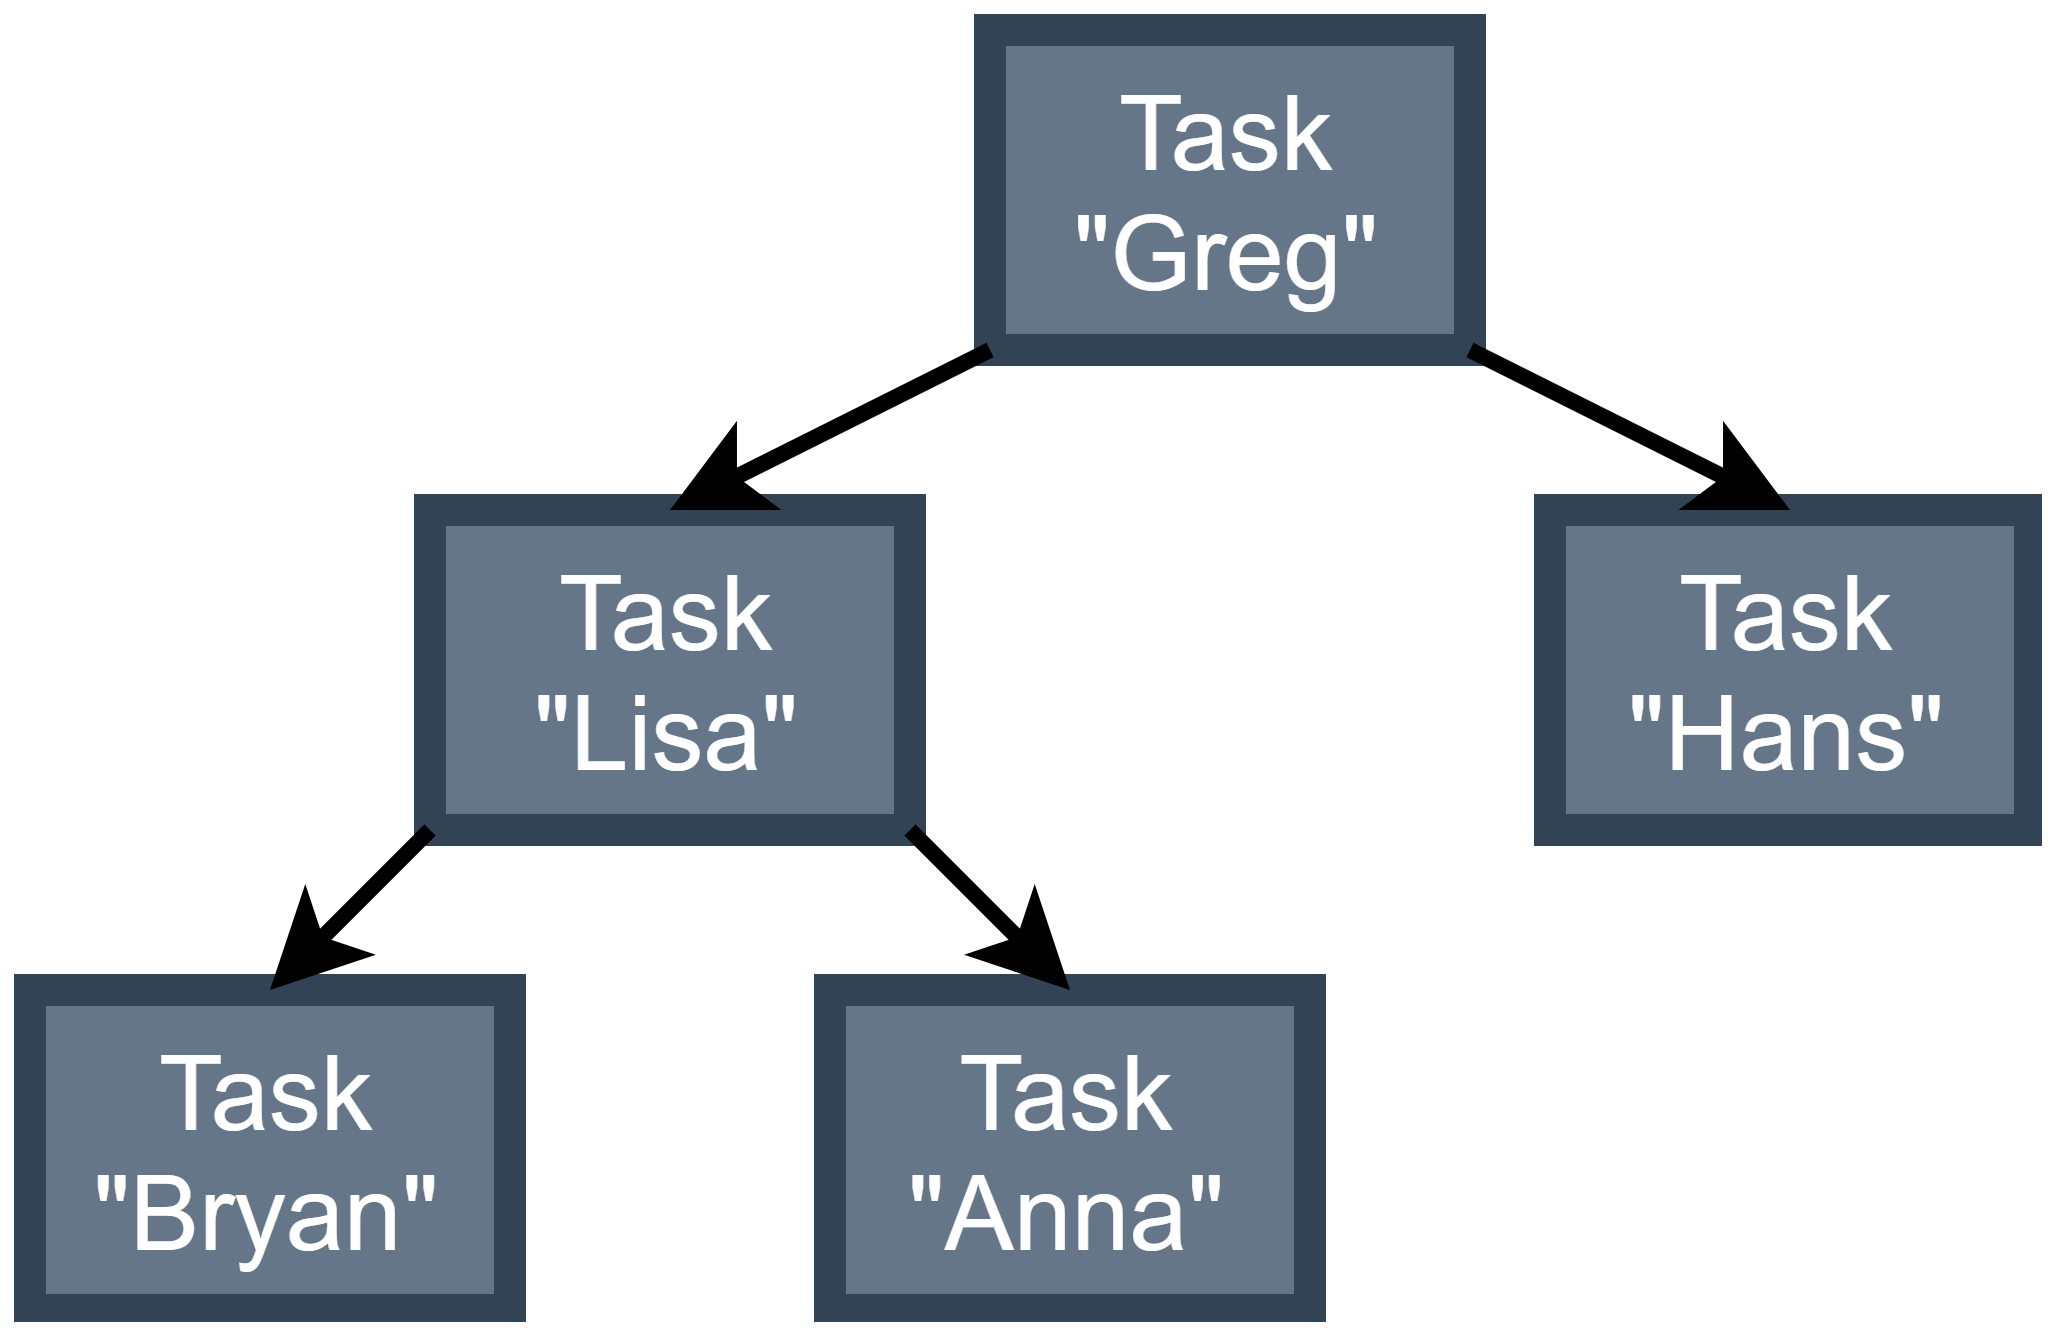
\includegraphics[width=1.0\linewidth]{img/structured-concurrency.png}
  \end{subfigure}
  \caption{Structured Concurrency}
  \label{Structured Concurrency}
\end{figure}
In this example, the main task called Greg will only continue once their sub-tasks Lisa and Hans are finished. Similar to that Lisa will only continue once Bryan and Anna are finished.
This structure can be nested as many times as necessary. Also, the main task can split into way more sub-tasks than in the example.
\\
Using structured concurrency makes the code-flow reliable and clear. This improves developing time. In order to implement structured concurrency a programming language needs to support several features, the most obvious being:
\begin{itemize}
  \item Tasks need to be able to spawn sub-tasks. There has to be a clear parent-child structure.
  \item Tasks need to be able to communicate whether they are done.
\end{itemize}

\cite{wiki:structured-concurrency}
\cite{loom:structured-concurrency}


\section{Code-Excerpts}
Project Loom is still under development. Therefore the code is still rough around the edges. Whenever code-excerpts are used in this thesis, they will be slightly altered:
\begin{itemize}
  \item Comments will be altered or removed for a better understanding of the reader.
  \item Any print outs used for debugging will be removed for the sake of clarity.
  \item Some parts of the code are experimental and exclusively used to monitor performance. Since they don't alter the actual way the program currently works, they are also removed for the sake of clarity.
  \item Correctness of any code in the JDK is extremely important. Even functions, that appear to be simple at first glance, have to be examined thoroughly. As an example, the rocket Ariane V crashed, because an Integer, which was supposed to be 64-Bit big, was saved as a 16-Bit one. The 16-Bit Integer did not have enough space to represent the Value of the variable correctly, which resulted in a crash.\cite{Ariane5} Therefore during development plenty of asserts are used to assure the correctness of the code. For example in the following code-excerpt the assert is used to assure, that the semaphore of a critical section never ends up being negative:

        \begin{lstlisting}[language=custom-java]
    public static void pin() {
      Continuation cont = currentCarrierThread().getContinuation();
      if (cont != null) {
          assert cont.cs >= 0;
          if (cont.cs == Short.MAX_VALUE)
              throw new IllegalStateException("Too many pins");
          cont.cs++;
      }
    }
    \end{lstlisting}

        Those asserts are also removed.
\end{itemize}

\section{Namechange}
Originally virtual threads were called fibers. In November 2019 project Loom decided to rename fibers to virtual threads. This decision was made due to multiple reasons:
\begin{itemize}
  \item First and foremost the name fiber made people think, that it is a new concept they would have to learn. This contradicts project Loom's core idea. The transition from kernel threads to virtual threads is envisioned to be an effortless process, which doesn't require relearning threads at all.
  \item Another reason is that the term fiber is connected to "superficially-similar-yet-essentially-different concepts"\cite{loom:namechange} elsewhere. 
\end{itemize}

\section{Java Profiler}
A Java profiler is a tool to monitor and analyze many components of a JVM during the execution of a program. As an example, it can monitor garbage collection and heap usage. There are many more things a Java profiler can monitor. Which values are monitored depends on the profiler one uses.
\subsection{VisualVM}
VisualVM is a clearly arranged Java profiler by Oracle. It is very easy to use and provides all the basic necessities. One can monitor heap size, heap usage and threads in detail. Unfortunately, VisualVM does not natively support exporting the collected data. Therefore plotting data collected with VisualVM oneself is not possible. \cite{Profiler:VisualVM}

\subsection{JProfiler}
JProfiler is another Java profiler by ej-technologies. It is much more powerful than VisualVM and allows the user to customize a lot of settings. The additional settings are of minor relevance to this thesis. The one feature that makes JProfiler a more attractive choice compared to VisualVM is the ability to export recorded data to a csv file. When only using the basic features, VisualVM and JProfiler look fairly similar on the surface. \cite{Profiler:JProfiler}
\begin{figure}[H]
  \centering
  \begin{subfigure}[b]{0.45\textwidth}
    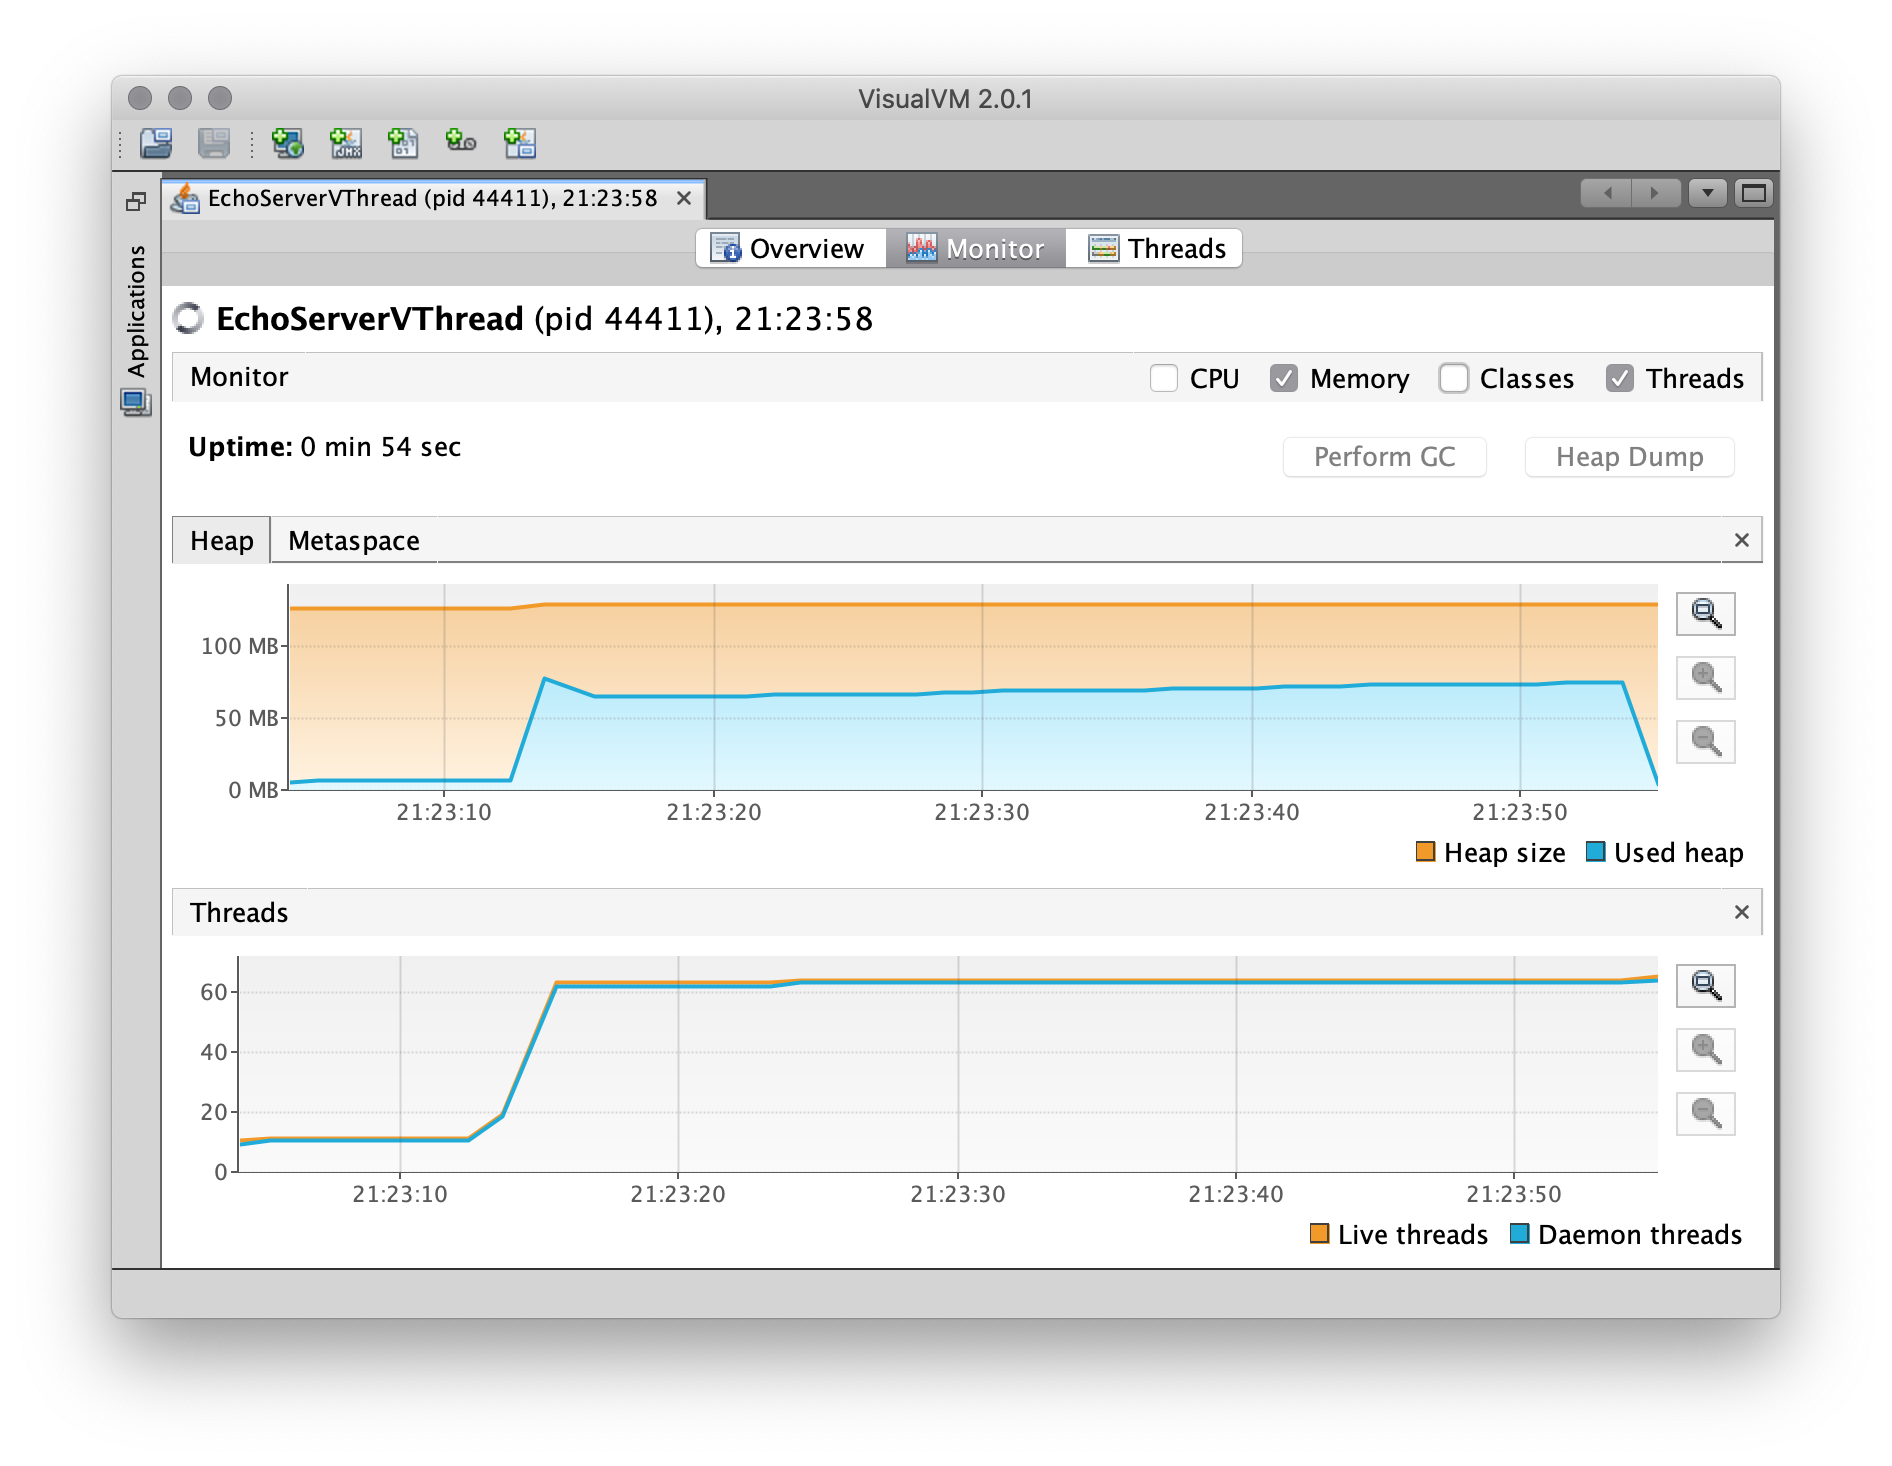
\includegraphics[width=1.0\linewidth]{img/visualvm-overview.png}
  \end{subfigure}
  \begin{subfigure}[b]{0.45\textwidth}
    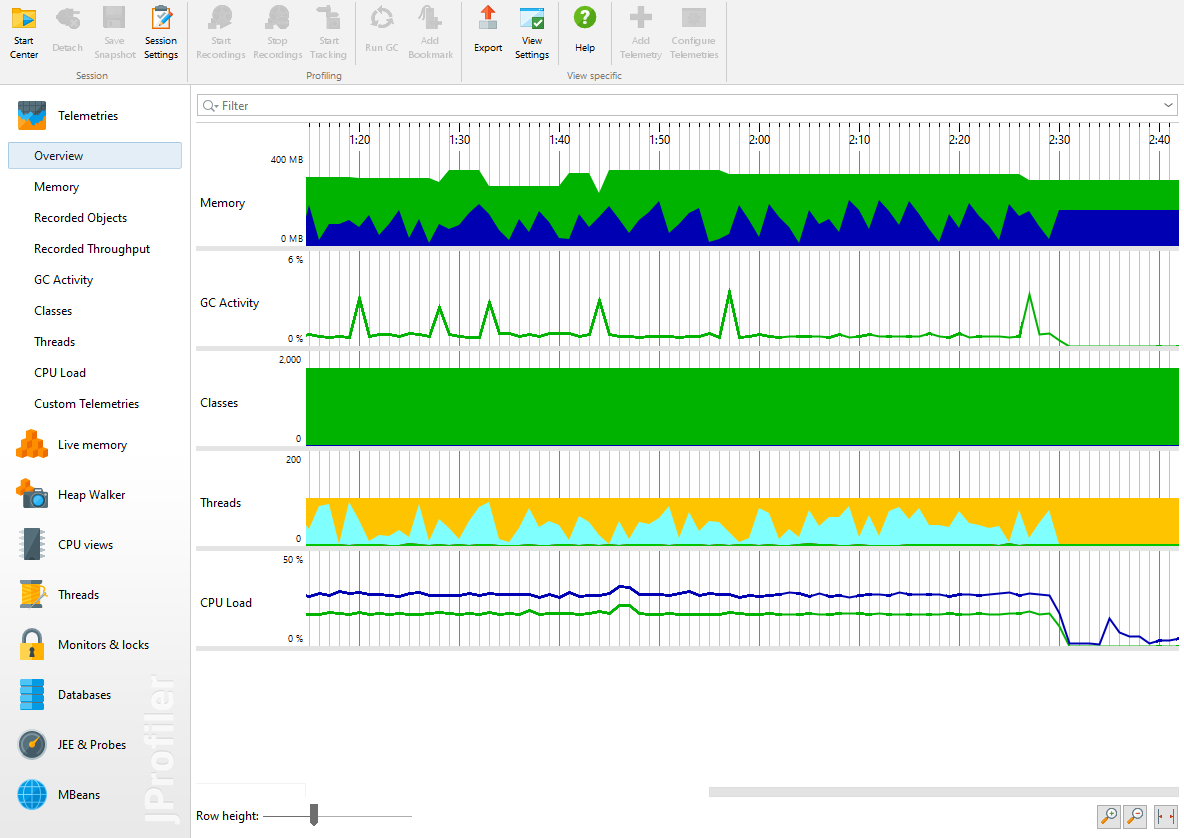
\includegraphics[width=1.0\linewidth]{img/jprofiler-overview.png}
  \end{subfigure}
  \caption{VisualVM - JProfiler - Side by side}
\end{figure}

\section{ApacheBench}
ApacheBench is a command-line utility part of the Apache HTTP Server Project, which is often abbreviated as Apache httpd. ApacheBench makes it possible to send many requests to a server to measure the time it takes to respond. It was originally designed to measure the performance of Apache servers, but it supports any other server just fine. It is very customizable. The flags most important to this thesis are used in the following example:
\begin{lstlisting}[language=no-numbers]
ab -n 1000 -c 10 -k http://localhost:5566/ 
\end{lstlisting}
This command will send 1000 requests to the server http://localhost:5566/. It will do so with a concurrency of 10. That means that 10 requests will be sent at a time. The -k flag enables the HTTP KeepAlive feature. Without it, every single request would start a new HTTP session. \cite{Apache:Bench}


\section{Java Microbenchmark Harness}
The Java Microbenchmark Harness is often abbreviated as JMH. It is a project of OpenJDK. They created it to benchmark JVMs. JVMs automatically make many optimizations to code. In general, this is very helpful, since it increases the performance. Unfortunately, it is not possible to turn off such optimizations. Therefore benchmarking Java programs is not an easy task.
\\
Benchmarks can be configured by using annotations. The most important annotations for this thesis are:
\begin{itemize}
  \item @BenchmarkMode
  \item @OutputTimeUnit
  \item @State
  \item @Warmup
  \item @Measurement
  \item @Fork
\end{itemize}
@BenchmarkMode defines what is measured. An example of that would be average time or throughput. @OutputTimeUnit defines how the measured results are returned. It can be any time unit, such as nanoseconds, seconds or minutes. Classes marked with the @State annotation are "instantiated on demand and will be reused during the entire benchmark trial" \cite{OpenJDK:jmh:3}. This annotation is a bit more complex, but most of the time it is used in a very simple manner: Just the benchmark class itself will be annotated with it. Then the JMH can reference its own fields just like any other Java program. This is called the default state. \cite{OpenJDK:jmh:4}
Typically the JVM is running a couple of Warmup runs before starting the actual benchmark. This is to be configured using the @Warmup annotation. Very similar to that the @Measurement annotation is used to configure the actual benchmark runs. Both support arguments like iterations. Which will tell the JMH how often to warmup or measure. There are two Fork options:
\begin{itemize}
  \item @Fork(0) = forking disabled
  \item @Fork(1) = forking enabled
\end{itemize}
Per default, JMH forking is enabled. Forking means that the tests will run in separate processes. This is done to avoid JVM optimizations. Often @Fork(1) is still annotated regardless, just for the sake of clarity. \cite{OpenJDK:jmh:12}
\\
\\
The OpenJDK JMH website provides information on building the projects. Any further explanation on how to use the JMH and its annotations is only provided in 38 sample Java files and the comments inside them. \cite{OpenJDK:jmh}

\section{Miscellaneous}
Project Loom is a big project with many people working on it daily. Therefore there are plenty of commits happening every single day. During this thesis, many different commits were analyzed. The code relevant to this thesis was mostly unchanged or was just slightly changed during writing it. The last commit used to analyze the code was committed on the 19.03.2020. The short hash-code for it is: 472bacfb77b
\\
\\
The code used in this thesis was run on all three major operating systems: Windows, macOS, Linux (Ubuntu 18.04 LTS in particular). The JDK used to compile and run is the same for all three: Build 15-loom+4-55, released on 22.02.2020.
\\
\\
All experiments in this thesis were run on the following environment:
\\
CPU: Intel i7 8700k
\\
RAM: 16GB
\\
OS: Ubuntu Desktop 18.04 LTS
\\
The JVM is always invoked without any additional flags.

